\documentclass[11pt]{article}
\usepackage[T1]{fontenc}
\usepackage{lmodern}
\usepackage[margin=0.92in]{geometry}
\usepackage{amsmath,amssymb,amsthm,mathtools,microtype}
\usepackage{tikz}
\usepackage[hidelinks]{hyperref}
\pdfinfoomitdate=1
\pdftrailerid{}
\pdfsuppressptexinfo=15
\hypersetup{pdftitle={A local characteristic precursor for the registered Einstein--scalar shell packet},
 pdfauthor={Ricardo Maldonado},pdfsubject={Working manuscript for author and specialist review}}
\newcommand{\dd}{\,\mathrm d}
\newcommand{\eps}{\varepsilon}
\newcommand{\norm}[1]{\lVert #1\rVert}
\newtheorem{proposition}{Proposition}
\newtheorem{premise}{Retained premise}
\title{A local characteristic precursor for the registered Einstein--scalar shell packet}
\author{Ricardo Maldonado\\Independent Researcher}
\date{5 November 2026\\[3pt]\small Working manuscript for author and specialist review}
\begin{document}
\maketitle
\begin{abstract}
We construct a short-past linear precursor of a registered compact
Einstein--scalar shell perturbation. The actual master data have nonzero
velocity. A fresh rational first-exit calculation verifies the static positive
collar and bounds the master potential at negative times by
$5500<\mathcal W<103000$. A backward Volterra construction then yields the
coupled first perturbation on $-1<x\le0$, before shell contact.
On every such Cauchy section, both normalized principal quadratic shares lie
strictly between $0.499999$ and $0.500001$.
On a characteristic half-diamond with interior past apex, the solution gives
two compatible past traces. Each exceeds $0.499999$ at its midpoint, whereas
their common corner value is below $-4\,10^{-8}$; each therefore has an
internal zero and is nonconstant. A second Volterra formula reconstructs the
same solution from these traces. This is a local linear construction and a
finite-interval obstruction to specified principal one-way data. It does not
select an earlier physical incoming state, complete a nonlinear null/shell
problem, or determine a second-order preparation.
\end{abstract}

\section{The fixed coupled packet and the question}
A compact packet supplied on a present Cauchy slice need not be a pure
traveling channel there. This fact alone says little about a more remote
incoming state: a potential or a shell can mix characteristic channels.
We examine a smaller, quantitative question for the registered packet:
what is its unique local linear past before shell contact, and what data
does it induce on two intersecting past characteristics?
The construction uses standard wave and Volterra methods. Finite-slab wave
estimates and time reversal are established tools~\cite{btw}; no new general
energy or characteristic principle is asserted.

The retained five-dimensional bulk action and one-copy outward shell laws are
\begin{equation}
\begin{aligned}
 S_{\rm bulk}&=\int\left(\frac R2-\frac{|\nabla\phi|^2}{2}
                                      -V_{\rm b}(\phi)\right)\dd\mu_g,\\
 {\rm Ric}_{AB}&=\partial_A\phi\,\partial_B\phi+\frac23V_{\rm b}g_{AB},
 &\Box_g\phi&=V_{\rm b}',&
 K^{\rm out}_{\mu\nu}&=\frac{\sigma}{6}\gamma_{\mu\nu},&
 n_{\rm out}\phi&=-\frac{\sigma'}2 .
\end{aligned}
\label{eq:action}
\end{equation}
Two identical interiors meet at a pure-tension shell.
The fixed model has
\begin{equation}
\begin{aligned}
 S(\phi)&=1-\phi+\phi^3/3,&
 V_{\rm b}&=(S')^2/2-2S^2/3,\\
 \sigma&=2S+10^{-3}(1+c_\sigma\phi),&
 c_\sigma&=\frac{96714321425692}{161839258930731}.
\end{aligned}
\end{equation}
The static spherical background, with unit three-sphere metric $\kappa$, is
\begin{equation}
 g_0=\dd y^2+\rho^2[-\dd t^2+\cosh^2t\,\kappa],
 \qquad \dd y=-\rho\dd z,\qquad
 a=\rho_y/\rho,\quad p=\phi_{0,y}.
 \label{eq:bg}
\end{equation}
The shell is $z=0$ and increasing $z$ points into the positive collar,
away from it. Write $\rho_b=\rho(0)$, $p_b=p(0)$ and $\eta=\phi_0-1$.
No measured SI scale is assigned to these model-normalized coordinates.

\begin{premise}
The actual smooth static branch, its selected analytic shell enclosure,
the all-point first master reconstruction, and its canonical and
common-harmonic one-jet identification are retained analytic inputs.
The fresh arithmetic below verifies a collar and potential enclosure from
those inputs. Hash authentication does not reprove the analytic identities
or an exact-family existence theorem.
\end{premise}

For the longitudinal first master $\mathsf V$, put
\begin{equation}
\begin{gathered}
 C=\rho(3a+2p_y/p),\quad
 \alpha=(\rho/\rho_b)^{3/2}p/p_b>0,\quad
 \alpha_z/\alpha=-C/2,\\
 \mathsf V=\alpha\cosh^{-3/2}t\,w,\qquad
 w_{tt}-w_{zz}+\mathcal W(t,z)w=0,\\
 \mathcal W=\frac{35}{4}\operatorname{sech}^2t-\frac{25}{4}
             +\frac{C_z}{2}+\frac{C^2}{4}+\frac23\rho^2p^2 .
\end{gathered}
\label{eq:master}
\end{equation}
The registered actual data are
\begin{equation}
\begin{aligned}
 w(0,z)&=q_\ell(z),& w_t(0,z)&=e^{-z}q_\ell(z),&
 \ell&=10^{-6},\\
 q_\ell(z)&=
 \begin{cases}
 \exp\!\left(4-\dfrac{\ell^2}{(z-\ell)(2\ell-z)}\right),
                                        &\ell<z<2\ell,\\
 0,&\text{otherwise}.
 \end{cases}
\end{aligned}
\label{eq:data}
\end{equation}
They are smooth and flat at the support endpoints. Their first velocity
is not zero. The native 31 October change concerned a second-response
approximation and does not change this first state~\cite{records}.
Set $x=t/\ell$, $r=z/\ell$, $U(x,r)=w(\ell x,\ell r)$, and
$Q(r)=q_\ell(\ell r)$. Then
\begin{equation}
 U_{xx}-U_{rr}+\mathcal VU=0,\quad
 \mathcal V=\ell^2\mathcal W(\ell x,\ell r),\quad
 U(0,r)=Q(r),\quad U_x(0,r)=\ell e^{-\ell r}Q(r).
 \label{eq:scaled}
\end{equation}
We retain the future-oriented definitions
$J_+=U_x+U_r$ and $J_-=U_x-U_r$. Their principal speeds are
$\dd r/\dd x=-1$ toward the shell and $+1$ away, respectively.

\section{Fresh negative-time coefficients on the actual collar}
\label{sec:coeff}
The selected wide-collar input declares $0\le z\le8\ell$, with outer box
\begin{equation}
\begin{gathered}
 129\le\rho\le131,\qquad -9/10^5\le\eta\le-8/10^5,\\
 -7/50000\le p\le-3/25000,\qquad
 111/1000\le a\le14/125.
\end{gathered}
\label{eq:box}
\end{equation}
This width is checked afresh; no narrower historical collar is enlarged
by assertion. Let $U_j=\partial_\eta^j V_{\rm b}(1+\eta)$. The static ODE is
\begin{equation}
 \rho_z=-\rho^2a,\qquad \eta_z=-\rho p,\qquad
 p_z=-\rho(U_1-4ap),\qquad a_z=\rho^{-1}+\rho p^2/3 .
 \label{eq:ode}
\end{equation}
Using the selected shell intervals and the actual polynomial
\begin{equation}
 V_{\rm b}(1+\eta)=-\frac2{27}+\frac{14}{9}\eta^2
   +\frac{50}{27}\eta^3-\frac{\eta^4}{6}
   -\frac49\eta^5-\frac2{27}\eta^6 ,
\end{equation}
the new rational verifier recomputes all four interval images and checks
\[
 I_{{\rm shell},j}+[0,8\ell]F_j(I_{\rm outer})
       \ \subset\ {\rm int}(I_{{\rm outer},j}) .
\]
All eight component margins are positive; also $131(8\ell)<9$, the
retained proper endpoint margin. The usual continuation/first-exit argument
therefore establishes \eqref{eq:box} on the declared static collar.
This is interval arithmetic on the ODE, not numerical integration or a
new sampled background orbit.

Writing $h=U_1/p$, direct substitution of \eqref{eq:ode} gives
\begin{equation}
\begin{aligned}
 C&=\rho(2h-5a),\\
 C_z&=\rho^2(2h^2-10ah+5a^2-2U_2-5p^2/3)-5,\\
 \mathcal W&=\rho^2\mathcal Q-\frac{35}{4}\tanh^2t,\qquad
 \mathcal Q=2h^2-10ah+\frac{35}{4}a^2-U_2-\frac{p^2}{6}.
\end{aligned}
\label{eq:potential}
\end{equation}
The polynomial and \eqref{eq:box} give exact strict guards
\begin{equation}
 \frac74<h<\frac73,\qquad \frac{31}{10}<U_2<\frac{25}{8},
 \qquad \frac13<\mathcal Q<6.
 \label{eq:scalarcaps}
\end{equation}
For example, expanding $U_1,U_2$ at $\eta=0$ and bounding each monomial
gives the rational comparisons
\[
 \mathcal Q>\frac{1933333317}{5000000000}>\frac13,\qquad
 \mathcal Q<\frac{2680267}{450000}<6.
\]
Since $|\tanh t|\le|t|$ for real $t$, \eqref{eq:potential} yields
\begin{equation}
 \begin{gathered}
 -\ell\le t\le0,\quad0\le z\le8\ell:
 \qquad5500<\mathcal W<103000,\\
 0<\mathcal V<\mu,\qquad \mu=\frac{103}{1000000000}.
 \end{gathered}
\label{eq:pastcap}
\end{equation}
Indeed $129^2/3-35\ell^2/4>5500$ and
$131^2\,6+35\ell^2/4<103000$.
The explicit time dependence uses the same positive-depth static branch.
No future five-mean operator cap, positive-time evolved error, or
physical negative-$z$ background is transferred to the past.

\section{The backward Cauchy solution before shell contact}
\label{sec:cauchy}
Fix $0<\tau<1$ and put $s=-x$.
The required support cone is
\begin{equation}
 1-s\le r\le2+s,\qquad0\le s\le\tau .
 \label{eq:support}
\end{equation}
It lies in $(0,3)$, inside the verified collar. Extend $\mathcal V$
smoothly to an auxiliary whole-line coefficient, unchanged near this
compact cone and with absolute bound at most $\mu$.
The solution constructed below is supported in \eqref{eq:support};
thus it is independent of this auxiliary extension. No physical
background outside the positive collar is introduced.

Write $\widehat U(s,r)=U(-s,r)$. The free backward wave and the actual equation are
\begin{align}
 \widehat U_f(s,r)&=\frac{Q(r-s)+Q(r+s)}2
        -\frac\ell2\int_{r-s}^{r+s}e^{-\ell y}Q(y)\dd y,\label{eq:free}\\
 \widehat U(s,r)&=\widehat U_f(s,r)-\frac12\int_0^s
       \int_{r-s+\xi}^{r+s-\xi}\mathcal V(-\xi,y)\widehat U(\xi,y)\dd y\dd\xi .
 \label{eq:volterra}
\end{align}
The minus sign in \eqref{eq:free} comes from the actual nonzero present
velocity in \eqref{eq:scaled}. On continuous functions with support
\eqref{eq:support}, the integral operator $K$ has norm at most
$\beta_\tau=\mu\tau^2/2<1$. Hence
$\widehat U=\sum_{n\ge0}(-K)^n\widehat U_f$ converges uniformly, constructs the solution,
and proves uniqueness and continuous dependence in this class.
Its tail after order $N$ is bounded by
$\beta_\tau^{N+1}(1+\tau\ell)/(1-\beta_\tau)$.
Differentiated Volterra equations give smoothness for the smooth compact
data and coefficient. Higher coefficient derivatives are bounded on
each fixed compact cone; they are not needed in the following norm bounds.

Here $\norm{\cdot}_2$ integrates in $r$ over the auxiliary whole line,
equivalently over the positive collar on this supported solution.
Translations and the $L^1$ norm of the interval convolution kernel yield
\begin{equation}
\begin{aligned}
 \sup_{0\le s\le\tau}\norm{\widehat U_f(s)}_2
     &\le(1+\tau\ell)\norm{Q}_2,&
 \sup\norm{\widehat U(s)}_2&\le B_\tau\norm{Q}_2,\\
 \sup|\widehat U|&\le B_\tau,&
 B_\tau&=\frac{1+\tau\ell}{1-\mu\tau^2/2}.
\end{aligned}
\label{eq:norms}
\end{equation}
For the pointwise bound use $0\le Q\le1$.
All these constants are bounded uniformly for $\tau<1$ by
\begin{equation}
 \beta=\frac\mu2=\frac{103}{2000000000}<1,\qquad
 B=\frac{1+\ell}{1-\mu/2}
       =\frac{2000002000}{1999999897}<1.000002 .
 \label{eq:B}
\end{equation}
Uniqueness identifies the solutions on overlapping closed slabs.
Their union gives the actual local linear solution on $-1<x\le0$.
Its support has a strictly positive shell gap at every such time.
For example the quarter-slab support lies in $[3/4,9/4]$ and the
half-slab support in $[1/2,5/2]$. The limiting front reaches $r=0$
only at $x=-1$. No endpoint interaction or earlier-past assertion is made.

\section{Persistence of both normalized principal channels}
\label{sec:shares}
Let $D_Q=\norm{Q_r}_2>0$. The two-endpoint Cauchy inequality on the
unit interval gives $\norm{Q}_2\le D_Q/2$.
Since $Q(3/2)=1$ and $Q(1)=Q(2)=0$, applying Cauchy separately to the
two half intervals also gives $D_Q^2\ge4$.
These analytic bump facts require no new bump sampling.
The initial norms of $J_\pm$ lie between
$(1-\ell/2)D_Q$ and $(1+\ell/2)D_Q$.
The exact characteristic equations are
\begin{equation}
 (\partial_x-\partial_r)J_+=-\mathcal VU,\qquad
 (\partial_x+\partial_r)J_-=-\mathcal VU.
 \label{eq:char}
\end{equation}
Translation preserves $L^2$. Their past integrals and
\eqref{eq:norms}--\eqref{eq:B} therefore imply
\[
 \norm{J_\pm(x)-\text{translated }J_\pm(0)}_2
 \le\mu|x|B\norm{Q}_2\le\frac{\mu B}{2}D_Q .
\]
Consequently, throughout $-1<x\le0$,
\begin{equation}
 (1-\delta)D_Q\le\norm{J_\pm(x)}_2\le(1+\delta)D_Q,\qquad
 \delta=\frac\ell2+\frac{\mu B}{2}
       =\frac{2206000103}{3999999794000000}<10^{-6}.
 \label{eq:delta}
\end{equation}
In particular neither channel vanishes on an entire such Cauchy slice.
For
$E_\pm(x)=\norm{J_\pm(x)}_2^2/4$, monotonicity of a ratio gives
\begin{equation}
 \frac{(1-\delta)^2}{(1-\delta)^2+(1+\delta)^2}
 \le\frac{E_\pm}{E_++E_-}\le
 \frac{(1+\delta)^2}{(1-\delta)^2+(1+\delta)^2}.
 \label{eq:ratio}
\end{equation}
The exact rational guards yield the simple strict display
\begin{equation}
 0.499999<\frac{E_\pm(x)}{E_+(x)+E_-(x)}<0.500001,
 \qquad -1<x\le0 .
 \label{eq:shares}
\end{equation}
Thus data with either $J_-=0$ or $J_+=0$ on an entire slice in this
interval cannot evolve into the registered data under the stated equation.
The unscaled $t,z$ weights differ by a common factor $1/\ell$, so their
shares agree. A spatially varying conjugation does not preserve these
weights. They are normalized-master principal quadratic diagnostics,
not physical canonical or Noether energies, radiation fluxes, or
conserved quantities in the variable-potential problem.

\section{Two compatible past characteristic traces}
\label{sec:diamond}
Use null coordinates $u=x+r$, $v=x-r$ and the half-diamond
\begin{equation}
 {\cal D}=\{1\le u\le2,\ -2\le v\le-1,\ u+v\le0\}.
 \label{eq:diamond}
\end{equation}
Its present base is the entire packet interval $x=0$, $1\le r\le2$.
Its past apex $A=(-1/2,3/2)$ lies inside the positive collar, not on
the shell. Its past faces are $u=1$ and $v=-2$.
They are not the shell-corner cut of the separate second-order
affine-null preparation discussion~\cite{records}.
Restrict the solution from Section~\ref{sec:cauchy} to define
\begin{equation}
\begin{aligned}
 f(v)&=U((1+v)/2,(1-v)/2),&-2&\le v\le-1,\\
 g(u)&=U((u-2)/2,(u+2)/2),&1&\le u\le2,\\
 c&=U(-1/2,3/2)=f(-2)=g(1).
\end{aligned}
\label{eq:traces}
\end{equation}
The common corner identity is exact; $c$ is not an independently
chosen zero. It is scalar trace compatibility for this local wave
problem, not full nonlinear null or shell compatibility.

\begin{figure}[htbp]
\centering
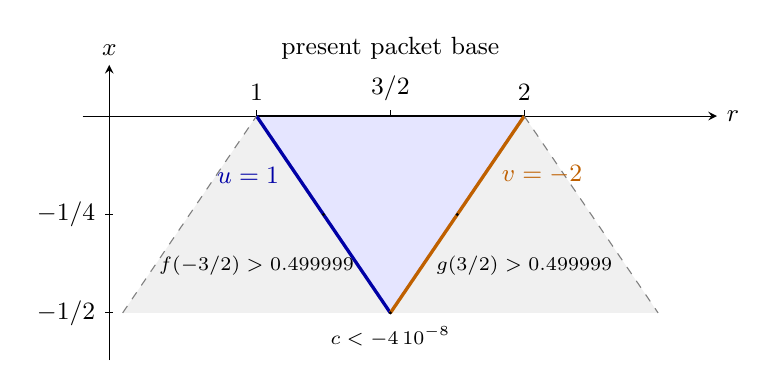
\begin{tikzpicture}[x=3.4cm,y=5cm,>=stealth,font=\small]
 \fill[gray!12] (1,0)--(2,0)--(2.5,-.5)--(.5,-.5)--cycle;
 \fill[blue!10] (1,0)--(2,0)--(1.5,-.5)--cycle;
 \draw[->] (.35,0)--(2.72,0) node[right] {$r$};
 \draw[->] (.45,-.62)--(.45,.13) node[above] {$x$};
 \draw[thick] (1,0)--(2,0);
 \draw[very thick,blue!65!black] (1,0)--(1.5,-.5);
 \draw[very thick,orange!75!black] (1.5,-.5)--(2,0);
 \draw[gray,dashed] (.5,-.5)--(1,0) (2,0)--(2.5,-.5);
 \foreach \r/\lab in {1/{1},1.5/{3/2},2/{2}} {
   \draw (\r,0)--(\r,.015) node[above] {$\lab$};}
 \draw (.435,-.25)--(.465,-.25) node[left,xshift=-3pt] {$-1/4$};
 \draw (.435,-.5)--(.465,-.5) node[left,xshift=-3pt] {$-1/2$};
 \fill (1.25,-.25) circle (.6pt);
 \fill (1.75,-.25) circle (.6pt);
 \fill (1.5,-.5) circle (.6pt);
 \node[blue!65!black,anchor=east] at (1.12,-.15) {$u=1$};
 \node[orange!75!black,anchor=west] at (1.88,-.15) {$v=-2$};
 \node[font=\scriptsize] at (1.0,-.38) {$f(-3/2)>0.499999$};
 \node[font=\scriptsize] at (2.0,-.38) {$g(3/2)>0.499999$};
 \node[font=\scriptsize,below] at (1.5,-.51) {$c<-4\,10^{-8}$};
 \node[above] at (1.5,.12) {present packet base};
\end{tikzpicture}
\caption{The actual characteristic half-diamond in $(r,x)$ coordinates.
The gray trapezoid indicates the half-time Cauchy support cone.
The two face midpoints are positive and their shared interior apex is
negative. The shell $r=0$ lies outside the diagram and is not contacted.}
\label{fig:diamond}
\end{figure}

Put $U_f(x,r)=\widehat U_f(-x,r)$. For the half slab let
\begin{equation}
 \beta_{1/2}=\frac\mu8,\qquad
 B_{1/2}=\frac{1+\ell/2}{1-\mu/8},\qquad
 \epsilon_*=\beta_{1/2}B_{1/2}
       =\frac{206000103}{15999999794000000}.
 \label{eq:eps}
\end{equation}
Equation~\eqref{eq:volterra} gives $|U-U_f|\le\epsilon_*$.
The free endpoint arguments at $(-1/4,5/4)$ are $1,3/2$, and those
at $(-1/4,7/4)$ are $3/2,2$. Hence
\begin{equation}
 f(-3/2),\,g(3/2)\ge\frac12-\frac\ell4-\epsilon_*
       >0.499999 .
 \label{eq:midpoints}
\end{equation}
At $A$ the two free displacement terms vanish, so
\[
 U_f(A)=-\frac\ell2\int_1^2 e^{-\ell r}Q(r)\dd r.
\]
On $[5/4,7/4]$, $Q\ge e^{-4/3}>1/4$. For instance the positive
Taylor sum and geometric tail give
\[
 e^{4/3}\le1+\frac43+\frac{(4/3)^2}{2}
       +\frac{(4/3)^3/6}{1-(4/3)/4}
       =\frac{103}{27}<4 .
\]
Together with $e^{-\ell r}\ge1-2\ell$, this proves
\begin{equation}
 c\le-\frac{\ell(1-2\ell)}{16}+\epsilon_*
       <-\frac1{25000000}=-4\,10^{-8}.
 \label{eq:corner}
\end{equation}
The negative corner depends on the registered nonzero velocity.
It would not follow from the same proof for zero initial velocity.

Each continuous trace therefore has an internal zero between its apex
and midpoint and is nonconstant. Each has a nonzero tangential derivative
somewhere on that half-face. Precisely,
\begin{equation}
 2f_v=J_-\quad(u=1),\qquad
 2g_u=J_+\quad(v=-2).
 \label{eq:factors}
\end{equation}
These are derivatives along the faces, not amplitudes transported in
the same direction as those faces.
Thus prescribing either face trace to be the constant $c$, or the
corresponding whole-face tangential principal derivative to vanish,
cannot produce this packet on $ {\cal D}$.
The zeros and sign changes survive positive smooth master conjugation
and orientation-preserving face reparametrization. Numerical channel
weights and derivative sizes do not remain unchanged under those operations.

In formulas with null arguments, $U(u,v)$ denotes
$U((u+v)/2,(u-v)/2)$. The wave equation is
$4U_{uv}+\mathcal VU=0$. Its Goursat formula is
\begin{equation}
\begin{aligned}
 U(u,v)=f(v)+g(u)-c-\frac14\int_1^u\int_{-2}^v
 \mathcal V((a+b)/2,(a-b)/2)U(a,b)\dd b\dd a .
\end{aligned}
\label{eq:goursat}
\end{equation}
Every integration rectangle stays inside $ {\cal D}$, and
$(u-1)+(v+2)\le1$ bounds its area by $1/4$.
The operator norm is therefore at most
\begin{equation}
 \frac\mu{16}=\frac{103}{16000000000}<1 .
 \label{eq:nullfactor}
\end{equation}
The convergent Volterra solution is unique and smooth for these compatible
smooth traces. It equals the previously constructed Cauchy solution and
reproduces both its present packet and its velocity.
This local two-face argument does not infer global retarded uniqueness
from one unrestricted null cut; such assertions need causal and
trace-space hypotheses~\cite{btw}.

\section{Coupled reconstruction, physical scope, and verification}
The master is not an unrelated test scalar. For the fixed sphere harmonic
$Y=n_1^2-n_2^2$, the retained differential reconstruction is
\begin{equation}
\begin{aligned}
 P&=\mathsf VY,\qquad \Psi=P/\rho^2,\qquad
 h_{yy}=-4\Psi,\qquad h_{y\mu}=0,\\
 h_{\mu\nu}&=2\Psi\,g_{0,\mu\nu},\qquad
 \delta\phi=-3P_y/(\rho^2p).
\end{aligned}
\label{eq:reconstruct}
\end{equation}
Here $\mu,\nu$ range over the four de Sitter directions in
\eqref{eq:bg}. Under the retained identities, \eqref{eq:master}
implies the full first linearized Einstein--scalar equations and
constraints. The same static ODE and smooth hyperbolic functions apply
on the verified negative-time domain.
For every compact past slab with $\tau<1$, all first-field jets vanish
on an open shell collar by \eqref{eq:support}. The physical first linear
junction rows are then background there. Identification with the fixed
common-harmonic representative still uses the full canonical one-jet,
including the mixed metric velocity, and the retained gauge/uniqueness
premises. No future gauge-error enclosure is used as a past error bound.

The characteristic data constructed here are restrictions of a selected
solution. They are not an independently selected physical state, arbitrary
incoming data, or an onto map to all prescribed histories. Their common
negative corner prevents interpreting them as two independently flat,
zero-corner bumps. A full nonlinear past problem must still supply and
propagate the other null constraints, the scalar equation, physical
shell conditions, and compatible free state data.
The constant-umbilic vacuum boundary theorem of
Fournodavlos--Smulevici~\cite{fs} is a useful comparison, but its homogeneous
boundary momentum-constraint mechanism does not by itself handle a
variable factor $\sigma(\phi)/6$ and scalar flux in five dimensions.

A conditional exact-family interpretation would additionally require a
time-reversed local development of an exact constraint curve and the
corresponding gauge identification. It is not proved by the linear
Volterra calculation. Higher-order constraint corrections can have a
larger support annulus than the first packet, so their contact-free
interval must not be inferred from \eqref{eq:support}.
No uniform effective nonlinear parameter window, second constrained
preparation, source or injected-energy law is obtained. Earlier incoming
states, potential scattering, or earlier shell interaction remain possible.
The result supplies no matter or radiation production, absolute proper
shell-observable sign, measured scale, or cosmological origin.

The accompanying exact verifier authenticates five local input copies:
two numeric enclosures and three selected analytic/state snapshots.
It recomputes four rational ODE images per successful process and the
potential, Volterra, channel, and trace guards. Normal and optimized
Python produce identical canonical reports. There are no project imports,
legacy checker calls, background/source/bump oracle queries, or numerical
PDE solves. Analytic reconstruction and branch premises remain explicit.
Independent coefficient and characteristic reviews, a displayed-bounds
audit, two fresh deterministic three-pass PDF builds, and all-page
visual review accompany this working manuscript.

\begin{thebibliography}{9}
\bibitem{btw}
C. B\"ar and R. Tagne Wafo, \emph{Initial value problems for wave equations
on manifolds}, Math. Phys. Anal. Geom. \textbf{18}, article 7 (2015),
\href{https://arxiv.org/abs/1408.4995v2}{arXiv:1408.4995v2}.
Theorem 8, Corollary 10, and Theorem 23 distinguish finite-slab control
from characteristic existence with causal hypotheses.

\bibitem{fs}
G. Fournodavlos and J. Smulevici, \emph{The initial boundary value problem
in General Relativity: the umbilic case},
\href{https://arxiv.org/abs/2104.08851v1}{arXiv:2104.08851v1}.
Theorem 1 and Lemma 1 concern a constant-umbilic four-dimensional
vacuum boundary; Appendix A treats scalar Robin estimates.

\bibitem{records}
R. Maldonado, \emph{Incoming preparation constraints and quadratic source
budgets for scalar shells}, working manuscript (4 November 2026),
\href{https://github.com/maldonado-research/HDblast/tree/main/research/HDBLAST_INCOMING_PREPARATION_LEDGER_20261104}{dated research capsule}.
The present capsule retains the selected source snapshots and records
the new past-domain calculation separately.
\end{thebibliography}
\end{document}
